\documentclass{article}
\usepackage[round]{natbib}

\usepackage{fullpage}
\usepackage{amsmath}
\usepackage{amsfonts}
\usepackage{graphicx}
\usepackage{color}

\usepackage{xr}
\externaldocument{supplement}

\newcommand{\aprcomment}[1]{{\textcolor{blue}{Comment: #1}}}
\newcommand{\E}{\mathbb{E}}

\title{Stabilizing selection, archaic introgression, and the distribution
of shared functional variation}
\author{APR}
\date{\today}

\begin{document}
\maketitle    

\begin{abstract}
    .
\end{abstract}

\section*{Introduction}

Genomic studies have shown that admixture is a common occurrance between
diverged populations and closely related taxa \citep{}, and potentially has
been widespread in primate \citep{} and hominin \citep{} evolution.
Understanding the effects of admixture on phenotypic and molecular variation is
therefore relevant to many natural systems, including to studies of the genetic
basis of complex traits and diseases. In particular, archaic introgression in
\emph{Homo sapiens} involving Neanderthals and Denisovans has recently
attracted considerable attention, both in understanding the historical
processes leading to observed distributions of introgressed DNA in present-day
populations \citep{prufer2014complete,villanea20??,chen2020identifying} as well
as its contribution to quantitative traits \citep{sankararaman,wei,others}.

After their introduction through admixture, introgressed alleles may be
selected either for or against. Some introgressed haplotypes appear to have
been positively selected in modern humans
\citep{huerta2014altitude,gower2021detecting,Enard}, possibly because such
alleles are locally adaptive and provide a fitness advantage when encountering
a novel environment. Despite these cases of adaptive introgression,
introgressed alleles were more likely to have been negatively selected in
modern humans \citep{harris2016genetic,juric2016strength}. As Neanderthal and
Denisovan population sizes are thought to have been relatively small for
hundreds of thousands of years, population genetics theory predicts that they
would accumulate deleterious variation at a faster rate than larger
populations.  Introgressed haplotypes would then carry more deleterious
variants, which would quickly be selected against after admixture. In mapping
the distribution of haplotypes identified as introgressed from Neanderthals,
there is a reduction of Neanderthal-related ancestry in enhancers and
regulatory regions
\citep{petr2019limits,telis2020selection,yermakovich2023long}. This
Neanderthal-allelic depletion, or ``deserts,'' support the hypothesis that
introgressed functional alleles were selected against
\citep{sankararaman2014genomic,sankararaman2016combined}.

There is genetic evidence that early \emph{H. sapiens} reciprocally contributed
to Neanderthal genomes \citep{kuhlwilm2016ancient,hubisz2020mapping}, with
introgression in the reverse direction occurring tens or hundreds of thousands
of years before the Neanderthal-to-human event surrounding the out-of-Africa
expansion around 60 thousand years ago (ka). This is supported by early ``near
modern'' \emph{H.  sapiens} outside of African around 120--100ka or earlier
\citep{schwarcz1988esr,grun2005u,beyer2021climatic}, potentially overlapping
with Neanderthals and providing opportunities for early contacts. While
estimates of the genomic contribution of early \emph{H. sapiens} to
Neanderthals vary \citep{}, up to XX\% of later Neanderthal genomes may have
been contributed through introgression from humans to Neanderthals. Under the
same argument that \emph{H. sapiens}-related haplotypes carry fewer deleterious
alleles, human-introgressed DNA may have been favored in Neanderthal genomes.
The replacement of Neanderthal mitochondrial and Y chromosomes by early human
haplotypes supports this model \citep{posth2017deeply,petr2020evolutionary}.

Models for selection on introgressed alleles are often based on load arguments
(in particular, differences in the rate of accumulation of unconditionally
deleterious variation in populations of different sizes) or hybrid
incompatibilities \citep{mueller,etc}. These arguments are founded primarily in
population genetics theory, eschewing any notion of genetic variation
contributing to phenotypic variation and selection operating on those
phenotypes. However, most phenotypic traits are thought to be under stabilizing
selection \citep{sanjak2018evidence}, including gene regulation
\citep{gilad2006natural,hodgins2015gene,price2022detecting}. This is especially
relevant for selection on Neanderthal-introduced alleles in modern humans, as
the strongest signals of selection against such alleles occur in regulatory
regions \citep{sankararaman2014genomic}.

Stabilizing selection on a trait acts to maintain the phenotypic distribution
of that trait near some trait optimum, which is achieved by reducing phenotypic
variation (Figure~\ref{fig:one-pop}A). When the mean phenotype of the
population is close to the phenotypic optimum, classical models predict that
alleles contributing to such a trait are subject to underdominant selection,
i.e., selection against the minor allele at a locus
\citep{robertson1956effect}. This has proven to be a useful model for
understanding allele frequencies of variants contributing to a trait under
stabilizing selection in the single-population setting
\citep[e.g.,][]{keightley1988quantitative, simons2018population,
hayward2022polygenic}.

\begin{figure}[tb!]
    \centering
    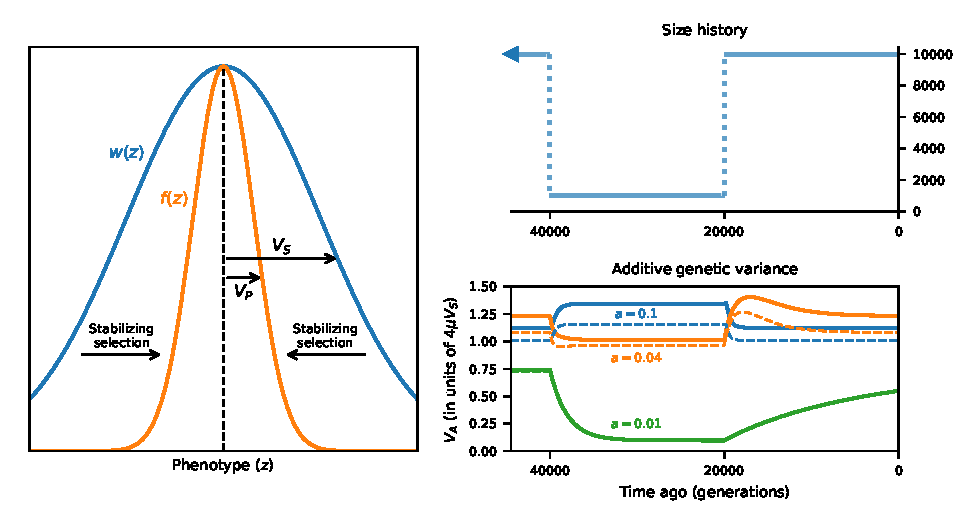
\includegraphics{../figures/one_pop.pdf}
    \caption{
        \textbf{Stabilizing selection and additive genetic variance in one population.}
        \aprcomment{See comparisons to simulations assuming free recombination in
        Figures~\ref{fig:one-popA}--\ref{fig:one-popC}.}
    }
    \label{fig:one-pop}
\end{figure}

In two diverged populations, the genomic architecture (i.e., mutations
underlying the trait) of a trait under stabilizing selection has a higher rate
of turnover compared to neutrally evolving loci \citep{yair2022population}. We
might therefore expect an accumulation of fixed differences between the
\emph{H. sapiens} and Neanderthal branches for alleles contributing to a trait,
even when the mean phenotype in each population is close to the same trait
optimum. When alleles that are fixed in one population are introduced to
another population in which they were previously absent, they will be at low
frequency and subsequently selected against. Likewise, if the ancestral allele
is reintroduced to a population fixed for a derived allele, the ancestral
allele will be at low frequency and will be selected against. In either case we
should expect the introgressed allele, whether ancestral or derived, to be
selected against, regardless the historical relative sizes of the populations
involved. This prediction contrasts with the population-genetics ``load''
model, in which haplotypes with fewer deleterious variants (such as those from
the population with larger historical size) are favored after introgression in
either direction.


\subsection*{Theory and model}

We consider a polygenic trait such that an individual's (additive) genetic
value is the sum over all effects of alleles in their genome, so that for
individual $i$, \(G_i = \sum_l g_{l, i} a_l\), where $a_l$ is the effect size
of the derived allele at locus $l$, and \(g_{l,i}\in\{0,1,2\}\) is their
genotype at that locus (i.e., the number of alleles they carry at that locus).
For unlinked loci, the expected additive genetic variance is \(V_A = \sum_l
2p_l(1-p_l)a_l^2\), where $p_l$ is the allele frequency at locus $l$. We ignore
dominance and epistatic effects, so that \(V_G = V_A\), assuming no linkage.
We can further ingore environmental effects \citep{simons2018population}, so
that the phenotypic variance \(V_P=V_A\).

Stabilizing selection acts to reduce phenotypic variation around the optimum
value $o$, and we assume a Gaussian fitness function so that relative fitness
is given by \(f(G_i | O, V_S) = \exp{(-(G_i - O) / 2 V_S)}\). $V_S$ can be
interpreted as the strength of selection on the trait, where larger $V_S$
implies weaker selection. For a population with mean phenotype at (or very
close to) the optimum, the mean fitness of the population (assuming a roughly
normal distribution of phenotypic values in the population) is
\[\bar{w} \approx \int_{-\infty}^\infty f(G | O, V_S) \mathcal{N}(0, V_G) dG
\approx \left(\frac{V_S}{V_S+V_G}\right)^{1/2}.\]
Thus, as the genetic variance increases, mean fitness among individuals in the
population decreases.

\subsubsection*{Mutation rates and effect sizes}

If all alleles contribute equally to the trait (as \(\pm a\)),
\citet{keightley1988quantitative} showed that the dynamics of $V_G$ can be
approximated with the recursion
\[V_{G,t+1} \approx V_{G,t}\left(1-a^2/2(V_S+V_G)\right)
\left(1-1/2N_e\right) + 2 \mu a^2,\]
where $\mu$ is the per-haploid, per-generation rate of mutation. In the
large-population-size limit, this gives the well-known results
\[\tilde{V_G} \approx 4\mu V_S,\] provided \(V_G \ll V_S\).
Mutations are not expected to each have the same effect size $a$, but
rather will be drawn from some distribution. Here, we will assume mutation
effect sizes are drawn from a normal distribution with mean 0 and given
variance $V_M$.

\subsubsection*{Approximating allelic dynamics via underdominance}

We model the distribution of allele frequencies underlying the trait using
the approximation that alleles are subject to symmetric underdominant selection.
For an allele with effect size $a$ (in the heterozygous state -- homozygotes
contribute $2a$ to the trait), the selection coefficient
\[s\approx \frac{a^2}{2(V_S + V_G)} \approx \frac{a^2}{2V_S},\]
if $V_G \ll V_S$ \citep[e.g.,][]{simons2018population}. Allelic dynamics can
be modeled using the diffusion approximation, where the expected change
in mean allele frequency per generation is
\[\E[M_{\delta_p}] \approx -s p(1-p)(1-2p),\]
and the expected change in variance of the allele frequency per generation is
\[\E[V_{\delta_p}] \approx \frac{1}{4N_e}p(1-p).\]
From this, because $s$ is always positive for any $a\not=0$, we see that
selection pushes allele frequencies to zero if $p<1/2$ and to one if $p>1/2$.
$p=1/2$ is an unstable equilibrium.

We extend the moments-based solution for the sample site-frequency spectrum
(SFS) \citep{jouganous2017} to include underdominance with given selection
coefficient $s$ (\(=a^2/2(V_S+V_G)\)). The contribution of alleles with effect
size $a$ to the total genetic variance $V_G$ is then found by computing the
expected pairwise diversity from the SFS (with sample size $n$, $\Phi_n$), as
\(V_{G,a} = 2a^2\sum_{j=1}^{n-1}\frac{j(n-j)}{n(n-1)}\Phi_n(j|a,\mu_a)da\).
Here, $\mu_a$ is the mutation rate of alleles with effect size $a$. The total
genetic variance is then \(V_G=\int_{-\infty}^\infty V_{G,a}
\mathcal{N}(0,V_M).\)

Figure~\ref{fig:one-pop}C shows that if $V_G$ is non-negligible compared to
$V_S$, ignoring $V_G$ and using $s=a^2/2V_S$ leads to lower estimates of
additive genetic variance. When mutation rates are large so that $V_G$ is not
small compared to $V_S$, using $s=a^2/2(V_S+V_G)$ provides estimates of $V_G$
that closely match simulations assuming free recombination between loci
(Figure~\ref{fig:toy-admixture}C,D). Because $V_G$ can change over time, this
means that $s$ is no longer constant, but can change due to factors such as
non-constant demography that increase or reduce $V_G$.

\begin{figure}[tb!]
    \centering
    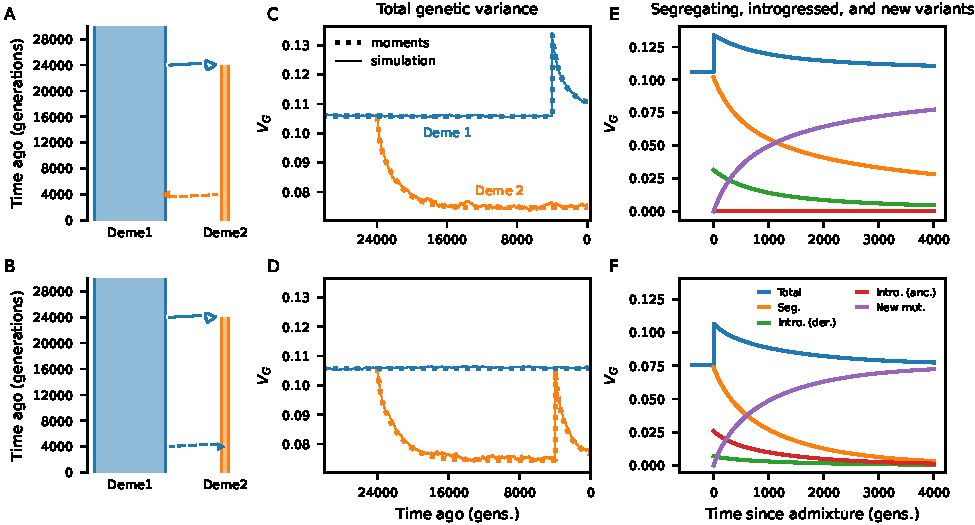
\includegraphics{../figures/reciprocal_admixture.pdf}
    \caption{
        \textbf{}
    }
    \label{fig:toy-admixture}
\end{figure}

\subsubsection*{Demographic history}

Our numerical solution for the SFS allows for non-constant population size
histories, population splits, continuous migration, and admixture. In this
study, we consider relativey simple scenarios involving population splits with
subsequent introgression events. We focus on parameter regimes relevant to
human-Neanderthal history. In the simplest model -- which is not meant to
perfectly match any particular known or inferred history, but instead
demonstrate the effect of reciprocal introgression following population
divergence -- a population of size $N_e=10\,000$ splits into two, on remaining
size $10\,000$ and the other shrinking to size $1\,000$. They remain isolated
for $2N_e$ generations (or 500 thousand years, assuming an average generation
time of 25 years) and then introgression occurs from one branch to the other,
contributing $5\%$ ancestry to the recipient population
(Figure~\ref{toy-admixture}A,B).

The second model is meant to more closely resemble inferred human-Neanderthal
history, in which the ancestral population of size $N_e=10\,000$ splits into
the human and Neanderthal branches. At 250ka, an early human-to-Neanderthal
introgression contributes $5\%$ ancestry to Neanderthals. The human branch
shrinks to size $1\,000$ 60ka, followed by exponential growth to $20\,000$ at
present time. Neanderthals contribute $2\%$ ancestry to this bottlenecked and
expanding human population at 50ka, after which their branch ceases
(Figure~\ref{fig:neand-to-human}A).

In each scenario, we track genetic diversity and phenotypic variance before and
after admixture to understand allele frequency and haplotype dynamics. The
trait optimum is $0$ in all branches, and the strength of selection $V_S=1$
remains constant.

\section*{Results}

\subsection*{Additive genetic variance after admixture}

We expect genetic variance to increase after introgression. The amount that
genetic variance increases depends on the allelic differences accumulated
between populations and the effects of those alleles. Assuming no linkage,
dominance or epistasis, \(V_G=\sum_l 2p_l(1-p_l)a_l^2\). After admixture, with
proportion $f$ contributed by the source population (labeled 0) into the focal
population (labeled 1), \(p_l = fp_{l,0} + (1-f)p_{l,1}\). Plugging into the
expression for $V_G$, and after some simple algebra (Appendix~AX), we can
express the expected genetic variance directly after admixture as \[V_G =
fV_{G,0} + (1-f) V_{G,1} + 2f(1-f)\sum_l F_{2,l} a_l^2,\] where $F_2 = (p_0 -
p_1)^2$ is the squared difference in allele frequencies at a locus
\citep[e.g.,][]{peter2016admixture}. This result in known \citep[e.g.,][]{},
showing that additive variance is equal to that in the source populations
weighted by their contributions, plus a term that depends on the divergence at
trait-affecting loci between the populations weighted by the quadratic factor
$2f(1-f)$.

In general, $F_2$ at a given locus will depend on the demographic history
relating the two populations and the effect size at the locus due to selection
on the trait. In the infinitesimal limit, involving many loci each of
vanishingly small effect, dynamics at a given locus will be approximately
neutral, so that $F_2$ depends only on the demography. In this case
\begin{align*}
    V_G & \approx f V_{G,0} + (1-f) V_{G,1} + 2f(1-f)\mathbb{E}[F_2] \sum_l a_l^2 \\
    & = f V_{G,0} + (1-f) V_{G,1} + 2f(1-f)\mathbb{E}[F_2] n_m V_M,
\end{align*}
where $V_M$ is the variance of effect sizes of new mutations (assuming the mean
is zero). 

For $a \not\approx 0$, assuming neutral evolution will tend to overestimate
$F_2$ compared to underdominant selection. We can compute expected $V_G$ both
before and after admixture using the diffusion approximation for the joint SFS
with underdominance. Comparing to simulations with free recombination between
loci (Appendix~AY), we find that this provides an excellent fit to average
observed $V_G$ over time (Figure~\ref{fig:toy-admixture}C,D). Following an
initial rapid increase in $V_G$ due to admixture, it decays back to the
steady-state expectation relatively rapidly.

\begin{itemize}
    \item Benefit of SFS -- partition by frequency classes (prev. seg vs introgressed)
    \item VG from all both previously segregating and introgressed alleles decays,
        replaced by VG due to new mutations
    \item Dividing VG from introgressed alleles into introduced derived vs reintroduced
        ancestral alleles shows the effect of differences in population sizes
\end{itemize}

\subsection*{Recurrent introgression and non-constant population size}


\begin{figure}[ht!]
    \centering
    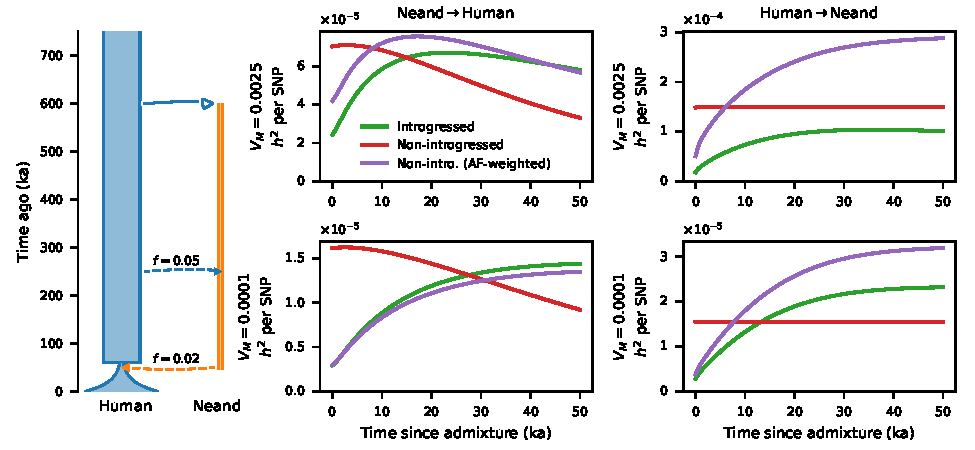
\includegraphics{../figures/neanderthal_admixture.pdf}
    \caption{
        \textbf{}
    }
    \label{fig:neand-to-human}
\end{figure}

\begin{figure}[ht!]
    \centering
    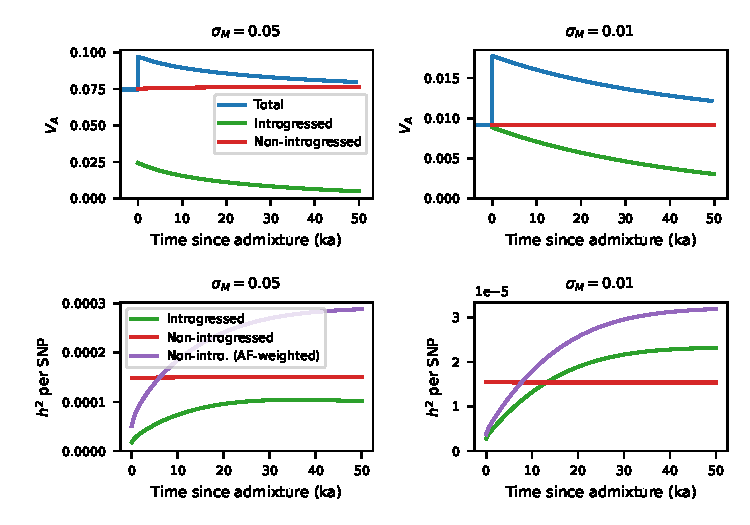
\includegraphics{../figures/human_admixture.pdf}
    \caption{
        \textbf{}
    }
    \label{fig:human-to-neand}
\end{figure}

\begin{figure}[ht!]
    \centering
    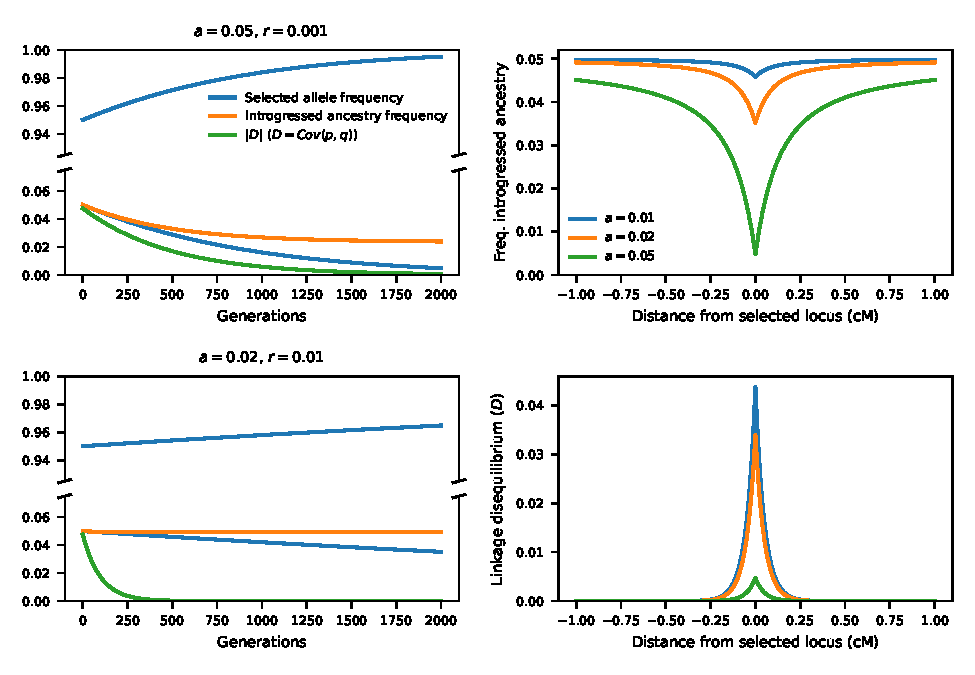
\includegraphics{../figures/linkage_predictions.pdf}
    \caption{
        \textbf{}
    }
    \label{fig:linkage-pred}
\end{figure}

\begin{figure}[ht!]
    \centering
    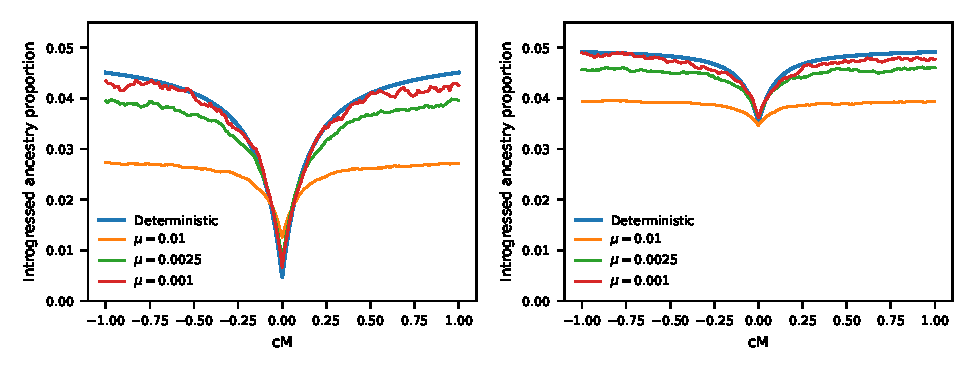
\includegraphics{../figures/linkage_simulation.pdf}
    \caption{
        \textbf{}
    }
    \label{fig:linkage-sim}
\end{figure}


\clearpage

\bibliographystyle{genetics}
\bibliography{manuscript}

\section{Appendix}

\subsection{Additive genetic variance after admixture}

Suppose two population (labeled 0 and 1) diverged some time in the past and
then admix in proportions $f$ and $1-f$.

Assuming no linkage, dominance or epistasis (so \(V_G=V_A\)),
\[V_G = \sum_l 2p_l(1-p_l)a_l^2 = \sum_l \pi_l a_l^2,\]
where $\pi$ denotes expected pairwise diverisity.
At a given locus (dropping the $l$), after admixture the allele frequency is
\[p=f p_0 + (1-f) p_1,\]
so that
\begin{align*}
    2p(1-p) & = 2(f p_0 + (1-f) p_1)(1 - f p_0 - (1-f) p_1) \\
    & = f^2 2p_0(1-p0) + (1-f)^2 p_1(1-p1) + 2f(1-f) (p_0(1-p_1) + p_1(1-p_0)) \\
    & = f^2 \pi_{0,0} + (1-f)^2 \pi_{1,1} + 2f(1-f)\pi_{0,1}.
\end{align*}

Plugging in to the definition for $V_G$, we get after admixture
\[V_G = f^2 V_{G,0} + (1-f)^2 V_{G,1} + 2f(1-f)\sum_l \pi_{0,1,l}a_l^2.\]
We can write $\pi_{0,1}$ at a given locus in terms of $\pi_{0,0}$, $\pi_{1,1}$,
and $F_2(0,1)=(p_0-p_1)^2$ as \citep{peter2016admixture}
\[\pi_{0,1} = F_2(0,1) + \frac{1}{2}\pi_{0,0} + \frac{1}{2}\pi_{1,1}.\]
Then
\begin{align*}
    V_G & = f^2 V_{G,0} + (1-f)^2 V_{G,1} + 2f(1-f)\sum_l \left[F_{2,l}(0,1)
    + \frac{1}{2}\pi_{0,0} + \frac{1}{2}\pi_{1,1}\right] a_l^2 \\
    & = f^2 V_{G,0} + (1-f)^2 V_{G,1} + 2f(1-f)\left[\frac{1}{2}V_{G,0} 
    + \frac{1}{2}V_{G,1} + \sum_l F_{2,l}(0,1)a_l^2\right] \\
    & = \left(f^2 + f(1-f)\right) V_{G,0} + \left((1-f) + f(1-f)\right)V_{G,1}
    + 2f(1-f) \sum_l F_{2,i}(0,1)a_l^2 \\
    & = f V_{G,0} + (1-f)V_{G,1} + 2f(1-f)\sum_i F_{2,l}(0,1)a_l^2.
\end{align*}


\begin{figure}[ht!]
    \centering
    %\includegraphics{}
    \caption{
        \textbf{Dynamics of additive genetic variance in two populations with admixture.}
        Coupled with the equations for the decay of $V_G$ due to drift and selection,
        and the increase in $V_G$ through mutation, show that the expected dynamics
        are matched by simulations without linkage.
    }
    \label{fig:VG_dynamics}
\end{figure}

\subsection{Dynamics of introgressed alleles}

\subsection{Reciprocal depletion of functional variation}

While incompatibilities require two or more loci (Morgan, 1942), introgression
with stabilizing selection can create the appearance of a single-locus
incompatibility via underdominance\dots

\subsection{The role of linkage}

\section{Discussion}

\section{Methods}

\end{document}
